\chapter{Evaluation}
\label{chap:eval}

I will begin by introducing test problems, against which I will evaluate the implementation. The subsequent section describes the hardware specification of the machines I tested the implementation on. The discussion about the results is in the last section with selected measurements. You can see complete results in Appendix \ref{chap:results}. The hyperparameters of the experiments are in Appendix \ref{chap:hyperparameters}.




%%%%%%%%%%%%%%%%%%
%%              %%
%%   PROBLEMS   %%
%%              %%
%%%%%%%%%%%%%%%%%%
\section{Problems Description}
\label{chap:problems}

For the \acrlong{acc:ga} experiments I used \acrshort{acc:sat} and \acrshort{acc:3sat} problems with various number of literals and clauses. The fitness function sums the number of unsatisfied (for minimization problem) or satisfied (for maximization problem) clauses. I implemented the fitness evaluation vectorized and fully in PyTorch, so the whole population is evaluated at once. I generated a new problem for every new experiment and all the problems were satisfiable. I achieved that by generating the assignment first and then generating the desired number of clauses. At least one literal in each clause matches the value with his corresponding counterpart in the previously generated assignment. Because I am more concerned with the running time of the algorithm rather than its performance, the satisfiability of the formulas does not make a big impact on the measurements.

The problem formula is kept as a matrix, where rows correspond to clauses and columns to indices of the literals. For a negative literal, the index is negative. This coding is efficient for \acrshort{acc:3sat} problem, but I run into a problem with generic \acrshort{acc:sat} problem with a diverse number of literals in the clause. Because the tensors in PyTorch need to be aligned in each dimension, I transform the generic \acrshort{acc:sat} problem into $k$-SAT problem, where $k$ is equal to the length of the longest clause. The shorter clauses duplicate their first literal, so their truth evaluation does not change, and all the clause has exactly $k$ literals. This may lead to a considerable inefficiency if the length variance between clauses is high. It may be worth to divide long clauses into smaller ones to reduce the overall size of the tensor and save some memory and computation. I believe this is not a serious obstacle for a broader application of the implementation.

The implementation processes files in the \textit{DIMACS CNF} format, which is the general and standard file format to define Boolean expression written in conjunctive normal form \citep{challenge1993satisfiability}. The evaluation and parser implementation, with the script to generates the problems, are in the attachment.

For the \acrlong{acc:pso} and real--\kern0.04em coded evolutionary algorithms I used well--established \acrfull{acc:coco} \acrfull{acc:bbob} test suite \citep{hansen2010comparing}. The suite consists of $24$ functions in $5$ groups with increasing difficulty. The groups vary in their separability, conditioning, unimodality, and global structure. It would not be feasible for me to measure the algorithms on all of them. Furthermore, as I am more interested in running time of the algorithm, there is no need to evaluate the implementation on all of them. The shifts in the running time would be caused primarily by the speed of the function evaluation rather than the algorithm itself.

The functions are randomly shifted in the search space. The $\mathbf{x}^{opt}$ specifies the position of the optimum. The optimum is always kept in the $\left[-5,5\right]$ interval in each dimension. Moreover, to eliminate the dependency of the algorithm on the absolute value of the function, it is shifted by the $f_{opt}$ value sampled from the Cauchy distribution with zero mean and scale equal $100$. This makes it difficult to directly use proportional--based selection operators because the optimum value differs each run and may be even negative. The algorithm does not know the $\mathbf{x}^{opt}$ and $f_{opt}$ values, and these are only used for the measurements. Except $\mathbf{x}^{opt}$ and $f_{opt}$, the functions may have other parameters (typically rotation matrices $\mathbf{R}$, $\mathbf{Q}$, diagonal scaling matrix $\Lambda$), that I do not describe here. Moreover, the functions may use functions to break symmetry ($T_{asy}^\beta$), penalize the parameters ($f_{pen}$), and add noise ($T_{osz}$). The exact definition is in the \acrshort{acc:bbob} specification \citep{hansen2010comparing}. These parameters are initialized randomly before each run. Lastly, the functions allow to specify their dimension $D$ at runtime, and the parameters are initialized accordingly. Therefore, it is easy to evaluate the algorithm on the same function with a different number of dimensions and hence on the problem with different difficulty.

I chose the following functions to evaluate the implementation. Not all the aspects of the algorithms were tested on all of these functions.
\begin{itemize}
    \item Function $f_1$ -- sphere function, that is unimodal, highly symmetric, rotationally and scale invariant. Sphere function is probably the simplest one, and can be easily solved using local search techniques.
    \begin{align*}
        f_{1}\left(\mathbf{x}\right) &= \norm{\mathbf{z}}^2+f_{opt} \\
        \mathbf{z} &= \mathbf{x} - \mathbf{x}^{opt}
    \end{align*}
    \item Function $f_7$ -- step ellipsoidal function. This function is unimodal, non--separable and has low conditioning. Because of the function step nature, it has many plateaus with zero gradient, so the gradient--based methods would not be very successful. Nevertheless, the function still exhibit ellipsoidal shape. 
    \begin{align*}
        f_{7}\left(\mathbf{x}\right) &= 0.1\max\left( \frac{\abs{\hat{z}_1}}{10^4}, \sum_{i=0}^D 10^{2\frac{i-1}{D-i}}z_i^2 \right) + f_{pen}\left( \mathbf{x} \right)+f_{opt} \\
        \hat{\mathbf{z}} &= \Lambda^{10}\mathbf{R} \left( \mathbf{x} - \mathbf{x}^{opt} \right) \\
        \tilde{z}_i &=\left\{ 
            \begin{array}{ll}
                \lceil 0.5 + \hat{z}_i \rceil       & \text{if}\ \hat{z}_i>0.5 \\
                \lceil 0.5 + 10\hat{z}_i\rceil / 10 & \text{otherwise}        \\
            \end{array}  
            \right. \\
        \mathbf{z} &= \mathbf{Q}\mathbf{\tilde{z}} 
    \end{align*}
    \item Function $f_{15}$ -- Rastrigin function, that is non--separable, have roughly $10^D$ local optima, low conditioning and global amplitude larger than local one. The function is highly multimodal and is not regular nor symmetric.
    \begin{align*}
        f_{15} &= 10\left( D-\sum_{i=1}^D \cos\left(2 \pi z_i\right) \right) + \norm{\mathbf{z}}^2+f_{opt} \\
        \mathbf{z} &= \mathbf{R}\Lambda^{10}\mathbf{Q}T_{asy}^{0.2} \left( T_{osz}\left(\mathbf{R}\left(\mathbf{z}-\mathbf{x}^{opt}\right)\right) \right)
    \end{align*}
    \item Function $f_{19}$ -- composite Griewank--Rosenbrock function. This function is highly multimodal and noisy.
    \begin{align*}
        f_{19}\left(\mathbf{x}\right) &= \frac{10}{D-1}\sum_{i=1}^{D-1}\left( \frac{s_i}{4000} - \cos\left(s_i\right) \right) + 10 + f_{opt}\\
        \mathbf{z} &= \max\left(1,\frac{\sqrt{D}}{8}\right)\mathbf{R}\mathbf{x}+0.5 \\
        s_i &= 100 \left(z_i^2 - z_{i+1}\right)^2 + \left(z_i-1\right)^2 \\
        \mathbf{z}_{opt} &= \mathbf{1}
    \end{align*}
    \item Function $f_{22}$ -- Gallagher's Gaussian 21--hi peaks function with 21 unrelated and random optima.
    \begin{align*}
        f_{22}\left(\mathbf{x}\right) &= T_{osz}\left( 
            10 - \max_{i=1}^{21} w_i \exp\left( -\frac{1}{2D}\left(\mathbf{x}-\mathbf{y_i}\right)^T\mathbf{R}^T\mathbf{C}_i\mathbf{R}\left(\mathbf{x}-\mathbf{y_i}\right) \right) 
        \right)^2 + \\
        & + f_{pen}(\mathbf{x}) + f_{opt} \\
        w_i &= \left\{
            \begin{array}{ll}
                1.1+8\frac{i-2}{19} & \text{for}\ i=2,\dots,21 \\
                10                  & \text{for}\ i=1 \\
            \end{array}
        \right.
        \\
        \mathbf{C}_i &= \Lambda^{\alpha_i} / \sqrt[4]{\alpha_i} \\
        \alpha_i &= \left\{ 
            \begin{array}{ll}
                \alpha_i = 10^6 & 
                    \begin{array}{l}
                        \text{for}\ i=1
                    \end{array} \\
                \alpha_i \in \left\{1000^{2\frac{j}{19}}|j=0,\dots,19\right\} &
                    \begin{array}{l}
                        \text{sampled randomly without} \\
                        \text{replacement for}\ i \neq 1
                    \end{array}
            \end{array}
        \right.
    \end{align*}
    \item Function $f_{24}$ -- Lunacek bi--Rastrigin function. This function is highly multimodal and deceptive, because of the promising area with local optima.
    \begin{align*}
        f_{24}\left(\mathbf{x}\right) &=
            \min\left( \sum_{i=1}^D\left(\hat{x}_i-\mu_0\right)^2, dD+s\sum_{i=1}^D\left(\hat{x}_i-\mu_1\right)^2 \right) + \\
            &+ 10\left(D-\sum_{i=1}^D \cos\left(2\pi z_i\right)\right)
            + 10^4 f_{pen}\left(\mathbf{x}\right) \\
        \hat{\mathbf{x}} &= 2 \text{sign}\left(\mathbf{x}^{opt}\right) \bigotimes \mathbf{x} \\
        \mathbf{x}^{opt} &= \mu_0 \mathbf{1}^{+}_{-} \\
        \mathbf{z} &= \mathbf{Q}\Lambda^{100}\mathbf{R}\left(\hat{\mathbf{x}}-\mu_0\mathbf{1}\right) \\
        \mu_0&=2.5,\mu_1=-\sqrt{\frac{\mu_0^2-d}{s}}, s=1-\frac{1}{2\sqrt{D+20}-8.2},d=1
    \end{align*}
\end{itemize}

I reimplemented all the \acrshort{acc:bbob} functions in PyTorch. They are fully vectorized so that the whole population can be evaluated at once. The implementation of these functions is in the attachment and is also available from PyPI as the \href{https://pypi.org/project/BBOBtorch/}{\textit{BBOBtorch}} package.




%%%%%%%%%%$%%%%%%%
%%              %%
%%   HARDWARE   %%
%%              %%
%%%%%%%%%%%$%%%%%%
\section{Hardware Specification}

I run all my experiments in \href{https://metavo.metacentrum.cz/en/}{MetaCentrum}. I used servers with specifications in Table \ref{tab:cpuspec} for workloads running on \cpuns. For \gpu specialized tasks, I used servers with hardware specifications in Table \ref{tab:gpuspec}.


\begin{table}[t]
    \begin{subtable}[b]{0.4\textwidth}
        \begin{tabular}[b]{|l|l|}
            \hline
            CPU     &   AMD EPYC\texttrademark\ 7452 \\
            \hline
            RAM     &   $256$ GiB \\
            \hline
            Disk    &   $2\times4$ TB HDD \\
            \hline
            Owner   &   \makecell{Faculty of Science,\\Charles University} \\
            \hline
        \end{tabular}
        \caption{Hardware specification for \acrshort*{acc:cpu} experiments}
        \label{tab:cpuspec}
    \end{subtable}
    \hfill
    \begin{subtable}[b]{0.55\textwidth}
        \begin{tabular}[b]{|l|l|}
            \hline
            CPU     &   Intel\textsuperscript{\textregistered} {X}eon\textsuperscript{\textregistered} Gold 5218 \\
            \hline
            RAM     &   $192$ GiB \\
            \hline
            Disk    &   $4\times240$ GB SSD \\
            \hline
            GPU     &   nVidia Tesla T4 \\
            \hline
            GPU memory     &   16GB \\
            \hline
            \cuda cores     &   2560 \\
            \hline
            Tensor cores     &   320 \\
            \hline
            Owner   &   CESNET \\
            \hline
        \end{tabular}
        \caption{Hardware specification for \acrshort*{acc:gpu} experiments\\}
        \label{tab:gpuspec}
    \end{subtable}
    \caption{Hardware specification of servers the implementation was tested on}
\end{table}

One drawback of using MetaCentrum is that the machines are shared amongst the academic community of the Czech Republic. I could not block the whole machine for a more extensive time because of the terms of use, moreover, it would not be morally right. I have done all the \cpu workloads using tasks with eight cores and all the \gpu workloads with two cores.

While some of the resources, for example \gpu and RAM, are allocated exclusively to the running task, other, for example disk, network bandwidth, and \cpu to some extent, are not. The \cpu situation is further complicated by the Hyper--Threading technology. This technology duplicates one physical processor core into two logical ones. While the first may use the full utilization of the core, the second one uses the idle portion of it. All the processors currently installed in the MetaCentrum, including the AMD EPYC 7452 processor, use this technology. As the goal of this work is focused on the computation quantity rather than on the raw computation power, experiments done on this second logical core may have a significant impact on the execution time, especially for the \cpu workloads. I did my best to mitigate this issue by allocating extra cores, running the experiments during unoccupied hours, and running the experiments on the same machine so that no other user could interfere. Nevertheless, the measurements may still be noisy.




%%%%%%%%%%%%%%%%%
%%             %%
%%   RESULTS   %%
%%             %%
%%%%%%%%%%%%%%%%%
\section{Results Discussion}

I run all the experiments on the hardware specified above, and because the \acrlong{acc:ea} are by their nature stochastic, I repeated each experiment a hundred times. The reported numbers are the mean of the given metric over these runs.

\definecolor{superlightgray}{gray}{0.92}
\vskip\baselineskip\noindent\colorbox{superlightgray}{\begin{minipage}{0.98\textwidth}
\leavevmode{\parindent=1em\indent} First \cuda call from the PyTorch runtime initialize the \cuda context and based on my measurements, it takes about $1.5$s. The initialization is done only once and it could add bias to the first run of the algorithm. I decided not to take the delay into account, and all the measurements in this work are without it. I would argue this delay is spread over the runs, and because of the stochastic nature of the \acrshort{acc:ea}, they should be executed multiple times in order to get reliable results.
\end{minipage}}
\vskip\baselineskip

The experiments run for the population of sizes $32$, $128$, $200$, $512$, $1024$, $2048$, $5000$, $10240$, $16384$, and $32768$ in the most cases. These values play a role in all the experiments and, most of the time, are the quantity shown on the $x$ axis. I show two types of results -- running time with respect to population size and fitness progress with respect to generations. Note that the second named needs to be taken with a grain of salt. Bigger population has advantage of more fitness evaluations (up to three orders of magnitude) and, therefore, it is in advantage. For practical application one needs to take into account not only the fitness, but also the running time of the algorithm.

Based on the experiments, the \cuda implementation seems to perform better from medium to big--sized problems and populations. That is not surprising, as the \gpu is intended for vast computation and memory demands. For small problems and populations, the runtime stays constant up to a certain threshold, where the runtime starts to increase linearly with the problem size. This is clearly visible in Figure \ref{fig:garunningtime} for \acrshort{acc:3sat} problem with $100$, $300$, and $800$ literals. In the case of $2000$ literals, I would already classify the problem as medium-sized. The time for even the smallest population of $32$ individuals is the same for both \cpu and \gpu implementation. Measurement of \acrshort{acc:3sat} problem with varying number of literals and clauses is depicted in Figure \ref{meas:garuntimeproblemsize} and the \gpu implementation clearly outperform the \cpu one over the whole domain. Note that I used a population size of $1000$ individuals, which is advantageous for the \gpu implementation.

\begin{figure}[t]
    \begin{subfigure}[t]{0.48\textwidth}
        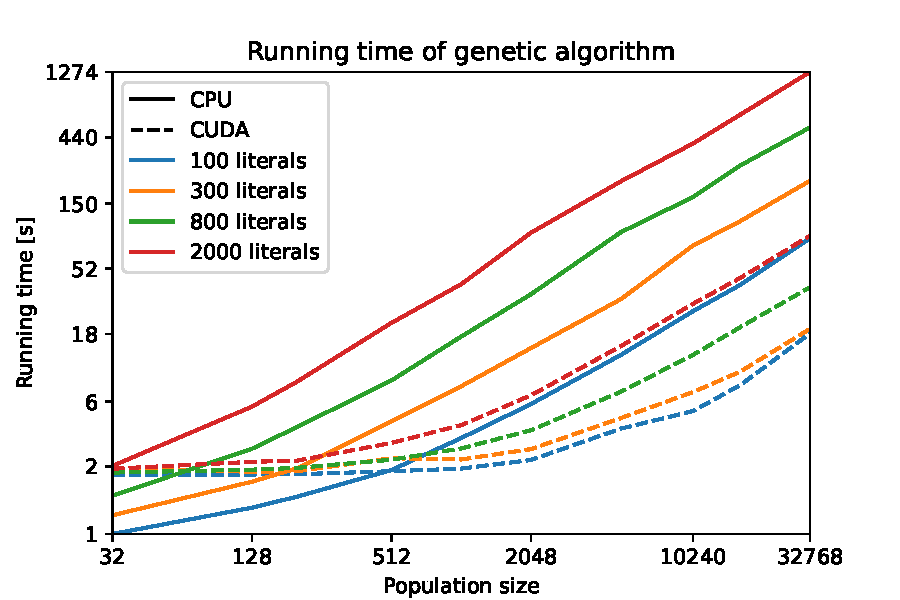
\includegraphics[width=\textwidth]{img/runs/time_ga_with_legend.pdf}
        \caption{Running time of \acrshort*{acc:ga}}
        \label{fig:garunningtime}
    \end{subfigure}
    \hfill
    \begin{subfigure}[t]{0.48\textwidth}
        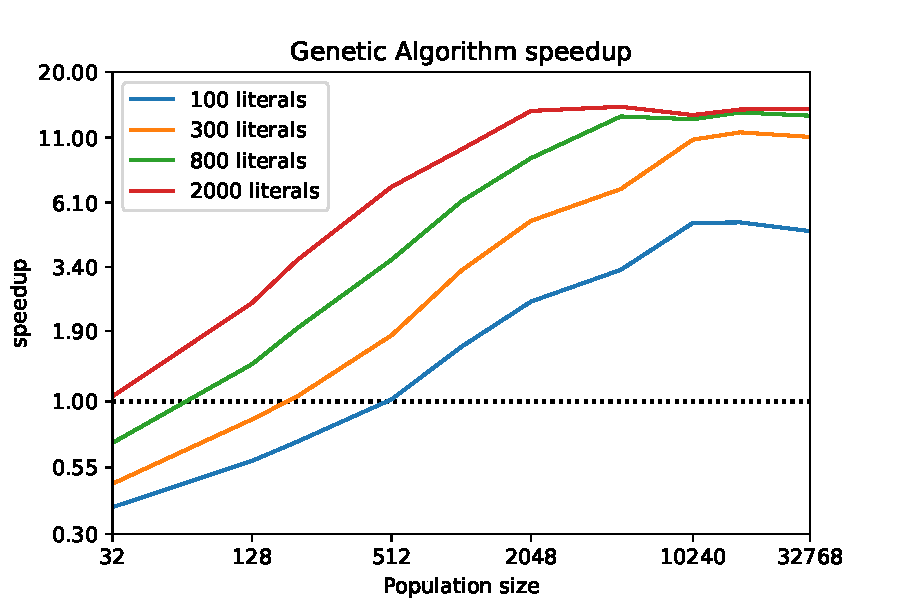
\includegraphics[width=\textwidth]{img/runs/speedup_ga.pdf}
        \caption{Speed up of \acrshort*{acc:ga} on \acrshort*{acc:gpu}}
        \label{fig:gpugaspeedup}
    \end{subfigure}
    
    \caption{\acrlong*{acc:ga} evaluation}
\end{figure}

The interesting observation is the constant run time of the \gpu implementation for small populations and problems. In these cases, the \gpu is not fully utilized, and the whole population can be processed truly in parallel. As the \cuda cores are less performant than \cpu cores, the total running time is higher than of \cpuns. Moreover, the communication overhead between \cpu and \gpu plays a relevant role in the running time. The speedup of the algorithm running on the \gpu is depicted in Figure \ref{fig:gpugaspeedup}.

I compared the PyTorch implementation to \cpp one in Figure \ref{fig:gapytorchvsc}. You can find the \cpp implementation in the attachment. It used master--worker architecture, where the fitness evaluation is done in parallel using multiple cores, whereas the rest of the algorithm is sequential. Both implementations use the same hyperparameters specified in Appendix \ref{chap:hyperparameters}. I compared the implementation using one and eight cores, along with the \gpu implementation. You may notice that \cpp implementation using one core outperforms PyTorch one by around $80\%$. Python is an inherently slow language, and the additional overhead of calling native code from Python underlines it. Moreover, the PyTorch implementation is a bit complicated compared to the simple \cpp implementation, which may also influence the running time. When I compared the implementations using eight cores, the difference is almost negligible (at most $20\%$). The PyTorch implementation took advantage of the parallelization of all the operators, and I believe an increased number of cores would further favor PyTorch implementation. The \gpu implementation still outperforms the \cpp implementation by order of magnitude on populations larger than five hundred individuals.

\begin{figure}
    \begin{minipage}[t]{0.48\textwidth}
        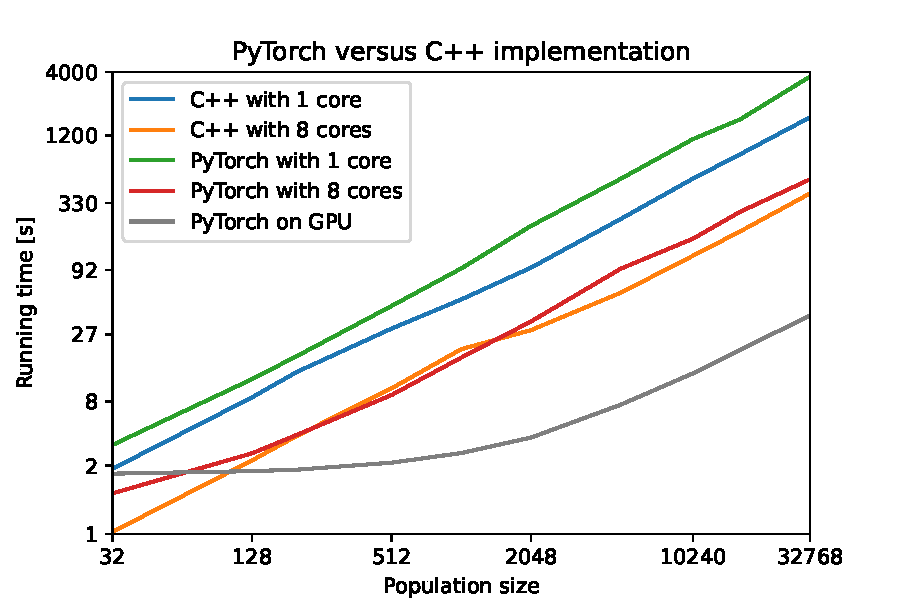
\includegraphics[width=\textwidth]{img/runs/time_ga_c_with_legend.pdf}
        \caption{Running time of C and PyTorch implementation}
        \label{fig:gapytorchvsc}
    \end{minipage}
    \hfill
    \begin{minipage}[t]{0.48\textwidth}
        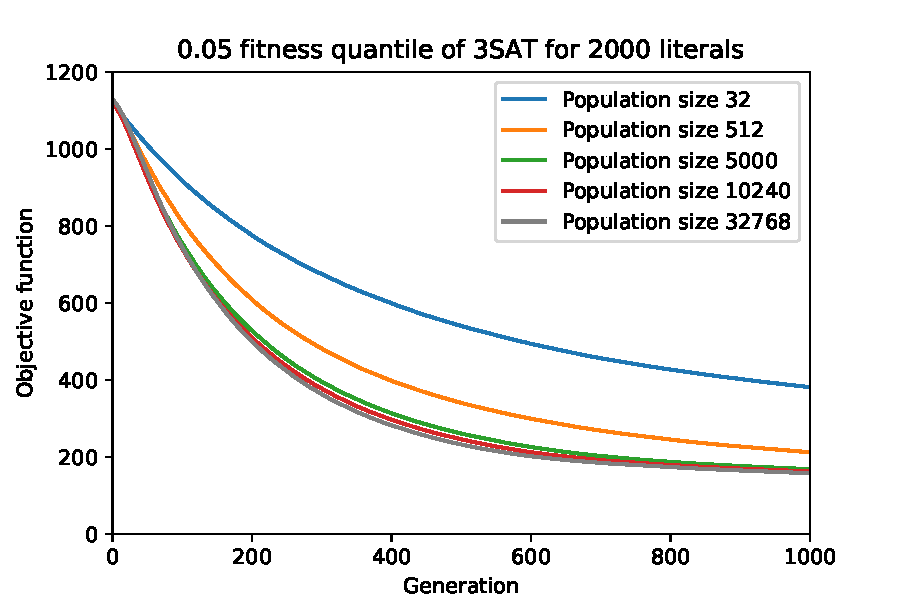
\includegraphics[width=\textwidth]{img/runs/fitness_ga_with_legend.pdf}
        \caption[Fitness of GA on 3SAT problem]{0.05 quantile of fitness on 3SAT problem with 2000 literals}
        \label{fig:gafitness}
    \end{minipage}

    \begin{minipage}[t]{0.48\textwidth}
        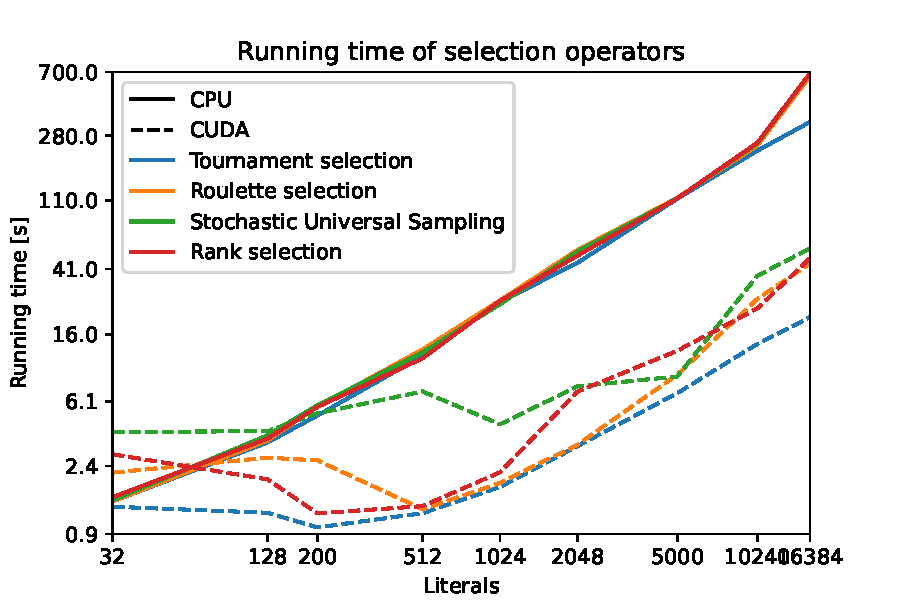
\includegraphics[width=\textwidth]{img/runs/time_ga_selections_with_legend.pdf}
        \caption{Running time of selection operators}
        \label{fig:selectiontime}
    \end{minipage}
    \hfill
    \begin{minipage}[t]{0.48\textwidth}
        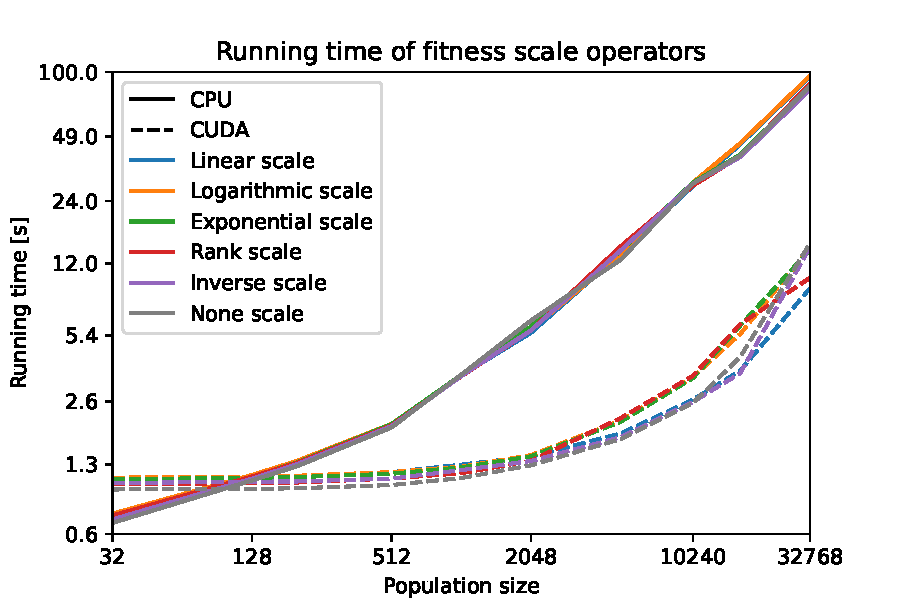
\includegraphics[width=\textwidth]{img/runs/time_ga_scale_100l_with_legend.pdf}
        \caption[Running time of fitness scale operators]{Running time of fitness scale operators for problem with $100$ literals.}
        \label{fig:gafitnessscaletime}
    \end{minipage}
\end{figure}


Of course, one would use a larger population only if it is advantageous. I measured the progress of fitness value over the generation, and these experiments are depicted in Figure \ref{meas:gafitness} (in Figure \ref{fig:gafitness} for $2000$ literals) and \ref{meas:gafitnesselite} (with elitism). I measured the $0.05$ quantile of the fitness function, and the algorithm converges faster for populations of size $32$, $512$, and $5000$. The big populations with $10240$ and $32768$ individuals do not make an impact until solving big enough \acrshort{acc:3sat} problem with $2000$ and $5000$ literals. Unfortunately, the improvement is not as significant as between the populations of size $512$ and $5000$. In my opinion, using that big population for this kind of problem is not worth it.

Running time of various selection operators is in Figure \ref{fig:selectiontime} (for \acrshort{acc:3sat} problem). Note that this is one of the more noisy experiments, although I repeat the experiment multiple times. For the \cpu implementation, the fitness evaluation is taking most of the time and the impact of the selection operator is scant. On the \gpu is the situation different, and the selection operators seem to have an order of magnitude difference. The fastest one is the tournament selection, which is not surprising, as it does not require sorting or search in the fitness array. On the other hand, the \acrshort{acc:sus} seems to be the slowest one, especially for smaller populations. For bigger populations of the size greater than $5000$ the performance of roulette, \acrshort{acc:sus} and rank selection looks very similar.

Lastly, I measured the impact of fitness scaling operators on the run time of the \acrshort{acc:ga}, and these results are in Figure \ref{fig:gafitnessscaletime} (experiments for $1000$ literals are in Figure \ref{meas:scale}). The algorithm used tournament selection, so the different scale operators did not influence the algorithm running time. Similarly to the selection, the fitness evaluation took the majority of the time, and the execution of the scale function does not make any impact when executed on \cpu (including the rank scale operator). The situation with \gpu was very similar except for a small problem ($100$ literals and $450$ clauses), where logarithmic, exponential, and rank scaling took slightly more time.

I tested mutation operators on real--\kern0.04em coded evolutionary algorithm with uniform crossover and tournament selection; the results for \acrshort{acc:bbob} function $f_{19}$ with $384$ dimensions is in Figure \ref{fig:esmuttime} (see Figure \ref{meas:muttime} for all the experiments). The fitness of normal and adaptive step mutations is in Figure \ref{fig:esmutfitness} (all the experiments are in Figure \ref{meas:mutfitness}). Both \cpu and \gpu implementations were slowest using Cauchy mutation. The reason is that the sampling from the Cauchy distribution lacks efficient implementation. The fastest was normal mutation with replacement mutation in some \gpu cases (on \cpu the replacement mutation was always a bit slower than the normal mutation). The adaptive step mutation was somewhere in between because of the fitness comparison overhead. The replacement mutation is interesting, as it outperformed normal mutation on some \gpu cases, but is steadily slower on \cpuns. I would say sampling a random value within an interval would be faster than sampling from the normal distribution and I cannot fully explain this.

\begin{figure}
    \begin{minipage}[t]{0.48\textwidth}
        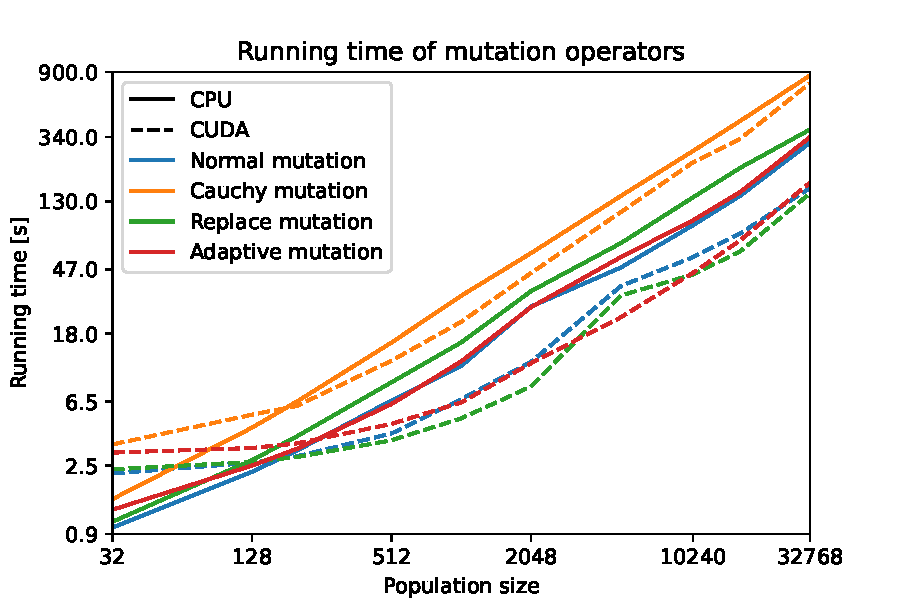
\includegraphics[width=\textwidth]{img/runs/time_es_mutation_with_legend.pdf}
        \caption[Running time of mutation operators]{Running time of mutation operators for \acrshort{acc:bbob} function $f_{19}$ with $384$ dimensions}
        \label{fig:esmuttime}
    \end{minipage}
    \hfill
    \begin{minipage}[t]{0.48\textwidth}
        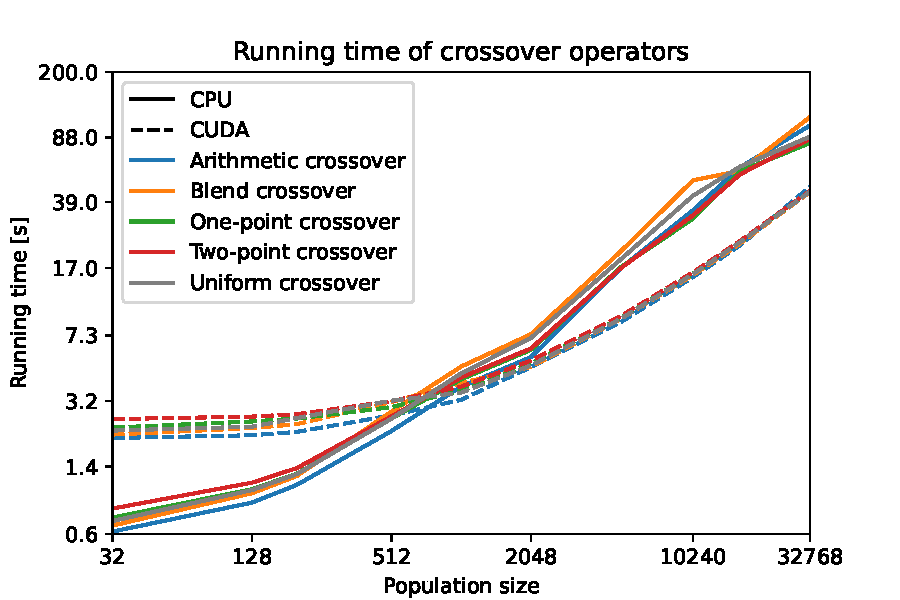
\includegraphics[width=\textwidth]{img/runs/time_es_crossover_with_legend.pdf}
        \caption[Running time of crossover operators]{Running time of crossover operators for \acrshort{acc:bbob} function $f_{19}$ with $128$ dimensions}
        \label{ref:escrosstime}
    \end{minipage}
\end{figure}

\begin{figure}[ht!]
    \begin{subfigure}[t]{0.48\textwidth}
        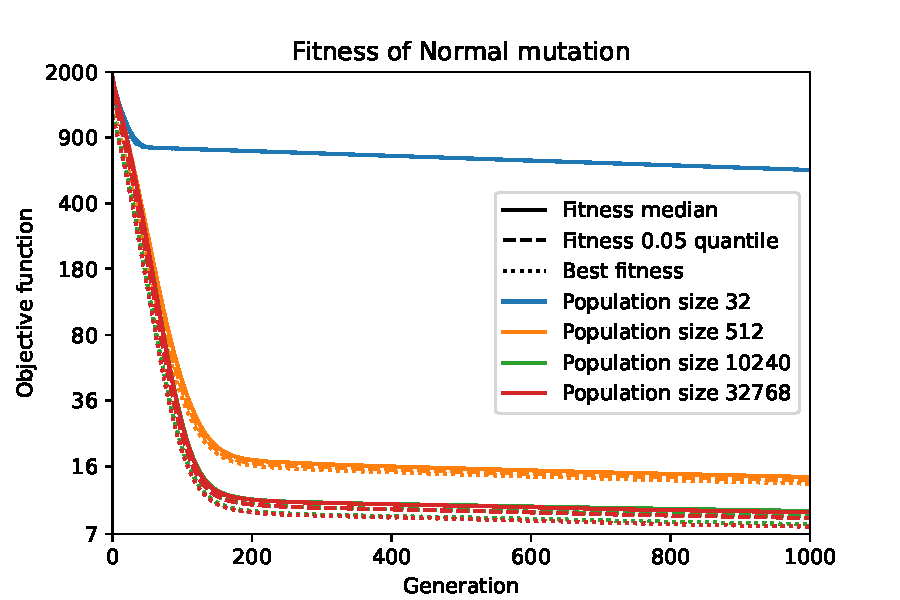
\includegraphics[width=\textwidth]{img/runs/fitness_es_mutation_AddFromNormal_with_legend.pdf}
    \end{subfigure}
    \hfill
    \begin{subfigure}[t]{0.48\textwidth}
        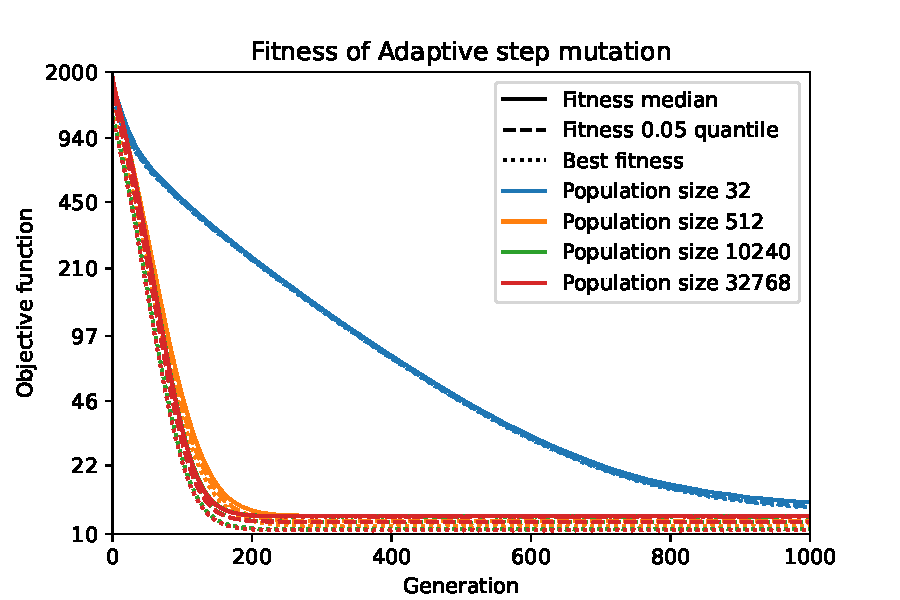
\includegraphics[width=\textwidth]{img/runs/fitness_es_mutation_AdaptiveStep_with_legend.pdf}
    \end{subfigure}
    \caption[Fitness of mutation operators]{Fitness of normal and adaptive step mutation operators for \acrshort*{acc:bbob} function $f_{19}$ with $384$ dimensions}
    \label{fig:esmutfitness}
\end{figure}

\begin{figure}[ht!]
    \begin{subfigure}[t]{0.48\textwidth}
        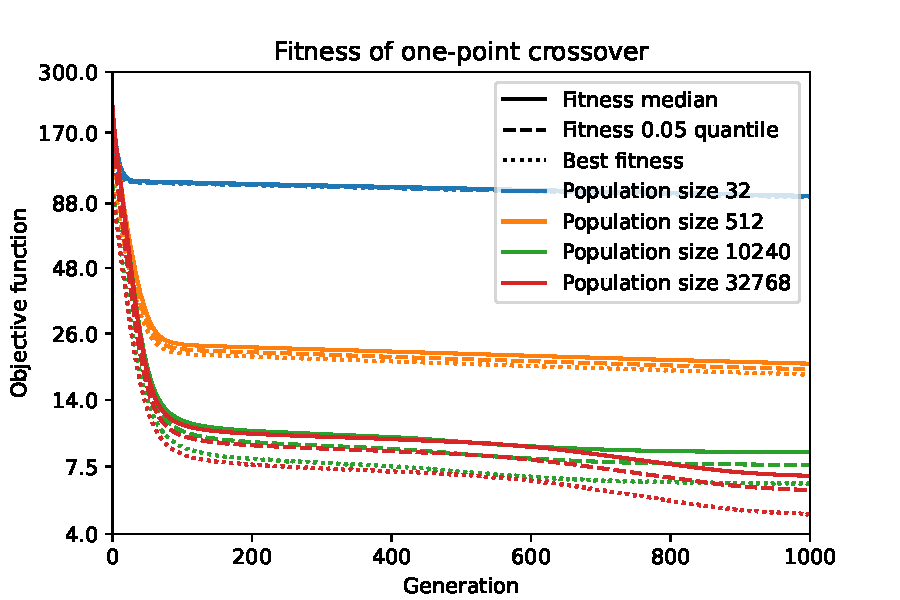
\includegraphics[width=\textwidth]{img/runs/fitness_es_crossover_OnePoint1D_with_legend.pdf}
    \end{subfigure}
    \hfill
    \begin{subfigure}[t]{0.48\textwidth}
        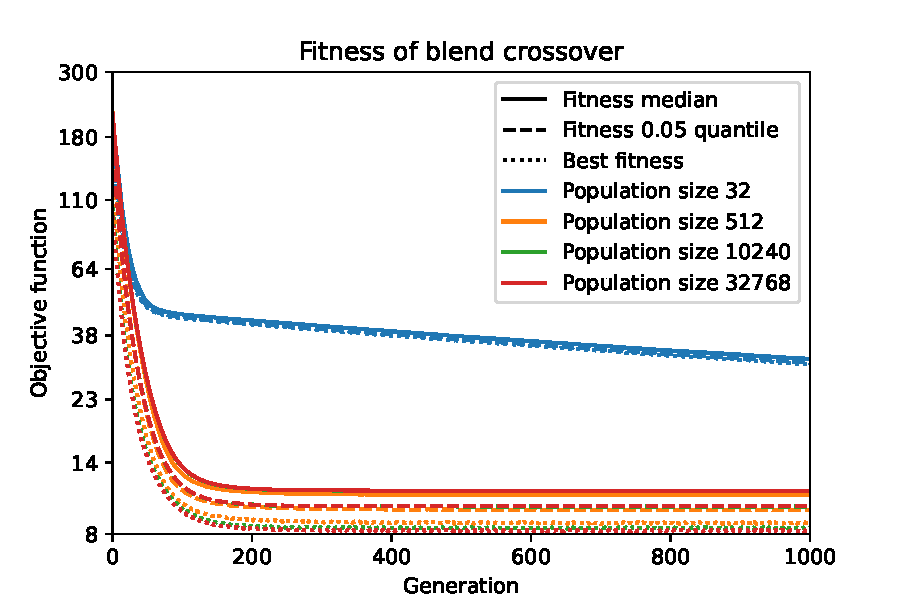
\includegraphics[width=\textwidth]{img/runs/fitness_es_crossover_Blend_with_legend.pdf}
    \end{subfigure}
    \caption[Fitness of crossover operators]{Fitness of one--step and blend crossover operators for \acrshort*{acc:bbob} function $f_{19}$ with $128$ dimensions}
    \label{fig:escrossfitness}
\end{figure}

From a convergence point of view, the complete experiments are shown in Figure \ref{meas:mutfitness}. The best performant mutation is the normal mutation, and as it is the fastest one, I would recommend it. Unfortunately, the various mutation operators do not take advantage of a bigger population, and except for population size $32$, the performance of populations with sizes $10240$ and $32768$ is the same. The algorithm converged a little faster with $10240$ individuals instead of $512$, but only for a problem with $384$ dimensions (see adaptive step mutation in Figure \ref{fig:esmutfitness}) and the difference is negligible. The only exceptions worth mentioning is the normal and Cauchy mutation for a problem with $24$ dimensions, where a larger population helped finding better optima. Bigger population also helped normal mutation in $384$ dimensions (see Figure \ref{fig:esmutfitness}), but this trend does not hold for population with $32768$ individuals. Lastly, you may notice better convergence properties of adaptive step mutation in contrast to normal or Cauchy mutation.

The crossover operators were tested on real--\kern0.04em coded evolutionary algorithm, and the running times are in Figure \ref{ref:escrosstime} (in Figure \ref{meas:crosstime} are all the experiments) along with their fitness values in Figure \ref{fig:escrossfitness} (complete experiments in Figure \ref{meas:crossfitness}). The running times were of the same order for all of them. The slowest on the \cpu was the blend crossover, while the arithmetic crossover was the fastest one. The slowest on the \gpu was the two--points crossover because of the complicated creation of the mask, as discussed in the Chapter \ref{chap:impl}. The fastest operator for small populations was the arithmetic crossover with the blend crossover. The running time for big populations on \gpu was almost identical for all the operators. Unlike mutation operators, some of the crossover operators take advantage of the larger population, as shown in Figure \ref{fig:escrossfitness} and \ref{meas:crossfitness} -- for example the one--point and two--point crossovers. On the other hand, blend crossover performed best using $512$ individuals, and a bigger population decreased its performance.

Lastly, the crossover schema experiments are depicted in Figure \ref{fig:esscemetime} (all experiments are in Figure \ref{meas:schema}). There is no surprise that the default schema (that is, the offspring replace their parents in the population) is the fastest one because it does not require extra memory allocation, as discussed in Section \ref{chap:gaimpl}. It is followed by comma schema, which is almost two times slower. The plus schema is the slowest and runs around $2.3$\kern-0.1em$\times$ slower than the default schema.

Finally, the running time of \acrshort{acc:spso2006} and \acrshort{acc:spso2011} algorithms are shown in Figure \ref{fig:psotime} (see Figures \ref{meas:spso2006time} and \ref{meas:spso2011time} for more details). The \acrshort{acc:pso} algorithm shows better speedup than \acrshort{acc:ga} and real--\kern0.04em coded evolutionary algorithms, even for problems with $384$ dimensions. The running times for problem with $6$, $32$, and $128$ dimensions is almost identical except the \acrshort{acc:bbob} function $f_{22}$. This function has the most complicated evaluation and it takes great portion of the running time. The graphs showing algorithm fitness for \acrshort{acc:bbob} function with $128$ dimensions is in Figure \ref{fig:psofitness} (more detailed experiments are in Figure \ref{meas:spso2006fitness} for \acrshort{acc:spso2006}, and in Figure \ref{meas:spso2011fitness} for \acrshort{acc:spso2011}). Unlike previous experiments, all the problems take advantage of the larger population, as is clearly visible in the figures. I would say the \acrshort{acc:pso} algorithm has the biggest potential to run on \gpuns.

\begin{figure}
    \begin{minipage}[t]{0.48\textwidth}
        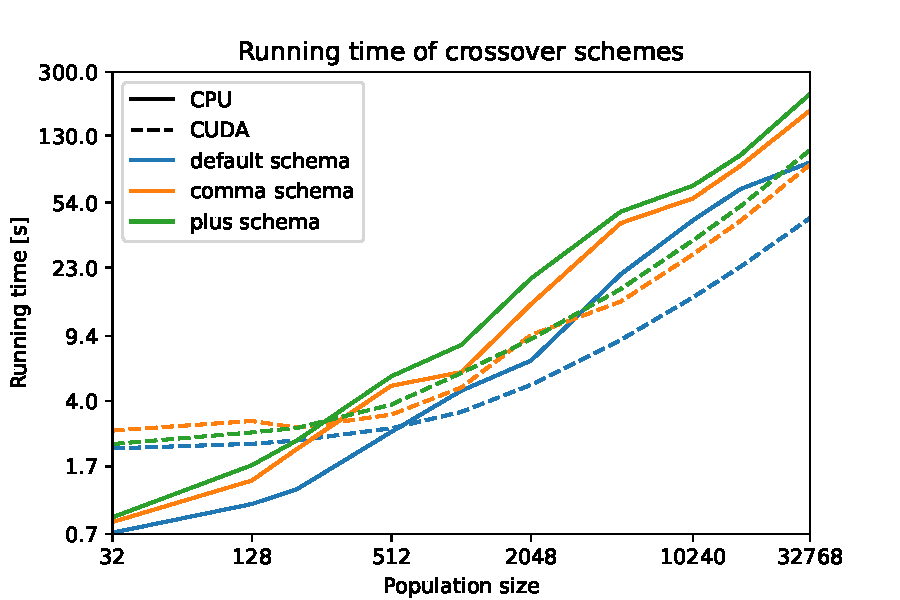
\includegraphics[width=\textwidth]{img/runs/time_es_schema_with_legend.pdf}
        \caption[Running time of crossover schemes]{Running time of crossover schemes for \acrshort{acc:bbob} function $f_{19}$ with $128$ dimensions}
        \label{fig:esscemetime}
    \end{minipage}
    \hfill
    \begin{minipage}[t]{0.48\textwidth}
        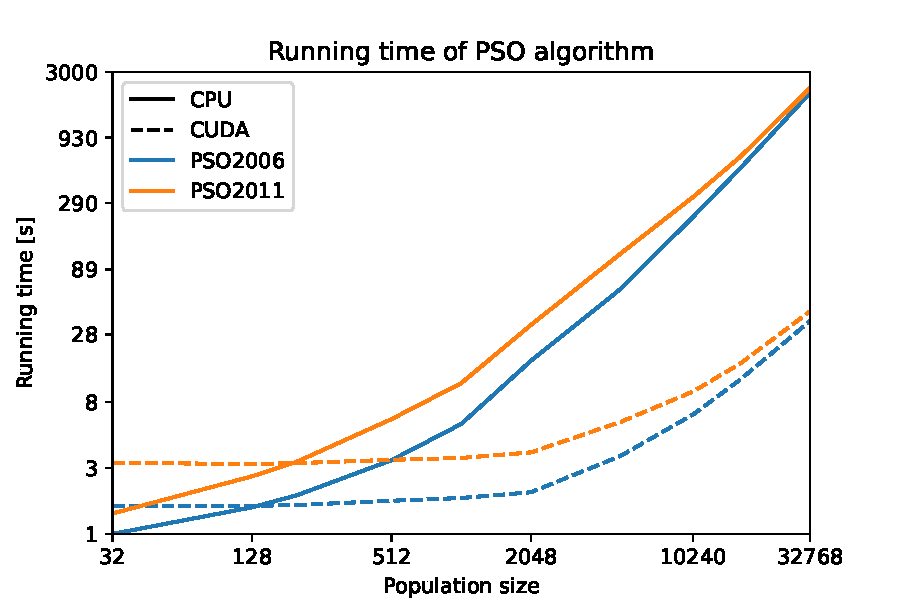
\includegraphics[width=\textwidth]{img/runs/time_pso_with_legend.pdf}
        \caption[Running time of \acrshort*{acc:pso}]{Running time of \acrshort{acc:pso} algorithm for \acrshort{acc:bbob} function $f_{19}$ with $384$ dimensions.}
        \label{fig:psotime}
    \end{minipage}

    \begin{minipage}[t]{0.48\textwidth}
        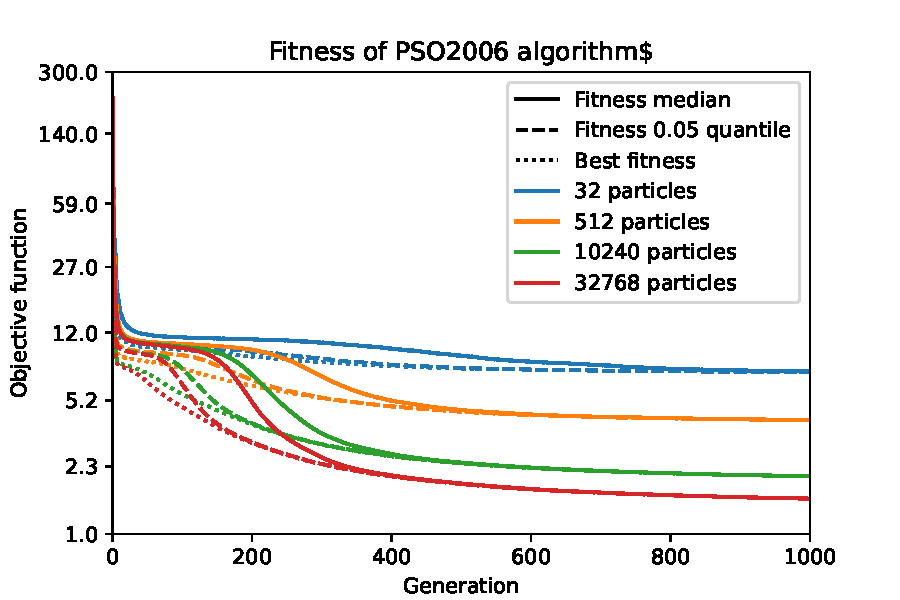
\includegraphics[width=\textwidth]{img/runs/fitness_pso2006_with_legend.pdf}
        \caption[Fitness of \acrshort*{acc:pso}]{Fitness of \acrshort{acc:pso} algorithm for \acrshort{acc:bbob} function $f_{19}$ with $128$ dimensions}
        \label{fig:psofitness}
    \end{minipage}
    \hfill
    \begin{minipage}[t]{0.48\textwidth}
        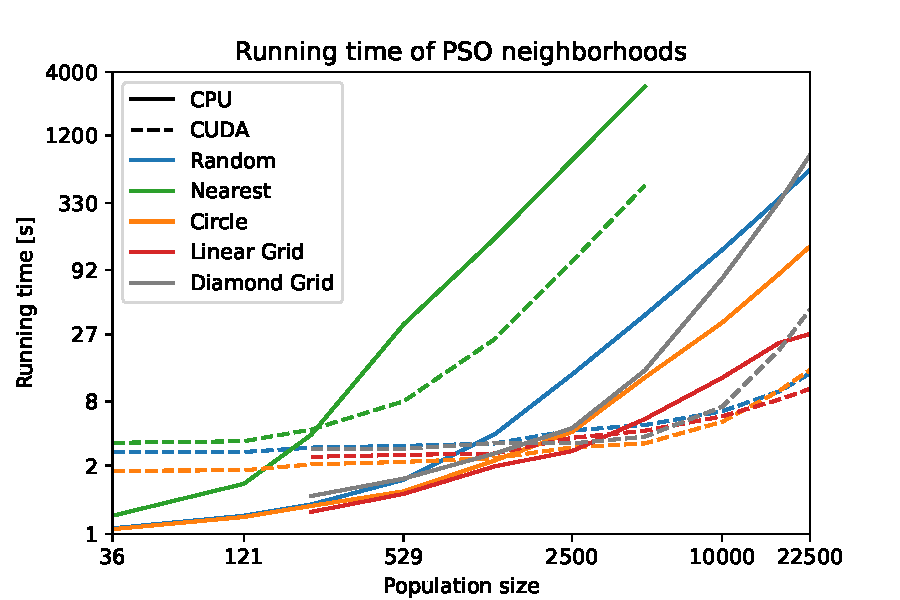
\includegraphics[width=\textwidth]{img/runs/time_pso_neigh_with_legend.pdf}
        \caption[Running time of \acrshort*{acc:pso} neighborhoods]{Running time of \acrshort{acc:pso} algorithm with  various neighborhood types for \acrshort{acc:bbob} function $f_{19}$ with $128$ dimensions.}
        \label{fig:psoneigtime}
    \end{minipage}
\end{figure}

The \acrshort{acc:pso} neighborhoods experiments are depicted in Figure \ref{fig:psoneigtime} (experiments for other \acrshort{acc:bbob} problems are in Figure \ref{meas:psoneigtime}), and the fitness is in Figure \ref{meas:psoneigfitness}. The random and circle neighborhoods are the fastest to evaluate on \gpuns, where the circle one is a bit faster for small populations. The circle neighborhood is static and generated only once, whereas the random neighborhood changes with every iteration. The random neighborhood is the slowest on the \cpu (except the nearest one) precisely for this reason. The grid--based neighborhoods are as fast as circle neighborhood for smaller populations, but for bigger populations the evaluation takes as long as random neighborhood. The cause is their substantial size in contrast to the circle one. The exception is the linear grid, which is the smallest of all the grid--based neighborhoods. 
Note that as circle and grid--based neighborhoods are static neighborhoods, their running time for the same neighborhood size should be equal.
The nearest neighborhood is extensively slower than any other. This is expected because it needs to measure the distance between every pair of particles, which is very costly even on \gpuns. The neighborhood evaluation is still more than six times faster on the \gpu for swarms larger than $500$ particles.

The overall statistics about the experiments are given in Table \ref{tab:totaltime}, including the number of experiments and the total running time. Note that some experiments failed, and I repeated some experiments to get more accurate measurements. The numbers, therefore, do not align to hundreds.

\begin{table}
    \centering
    \begin{tabular}{|l|r|r|}
        \cline{2-3}
        \multicolumn{1}{l|}{} & \textbf{\makecell{Number of\\experiments}} & \textbf{\makecell{Running\\time}} \\
        \hline
        \acrlong*{acc:ga} & $71\;068$ & $999.9$h \\
        Real--\kern0.04em coded evolutionary algorithms & $142\;866$ & $1136.8$h \\
        \acrlong*{acc:pso} & $195\;419$ & $1264.7$h \\
        Hyperparameter search & $7\;476$ & $49.5$h \\
        Testing runs & $5\;147$ & $53.5$h \\
        Failed runs & $30\;578$ & $136.6$h \\
        \hline
        CPU runs & $231\;352$ & $2567.6$h \\
        GPU runs & $221\;202$ & $1073.4$h \\
        CPUdays according to MetaCentrum & & $2149.2$h \\
        \hline
        Total & $452\;554$ & $3641.0$h \\
        \hline
    \end{tabular}
    \caption{Experiments running times}
    \label{tab:totaltime}
\end{table}